\chapter{Mathematical Model} % Main chapter title

\label{ch_math_model}

%----------------------------------------------------------------------------------------
%	SECTION 1
%----------------------------------------------------------------------------------------

\section{Assumptions/Problem Statement}

The turbine tower is modeled as a cantilever beam with a concentrated mass at the end.  The tower is the beam itself, and the nacelle is a concentrated mass at the end of the simplified beam.  The tower mass is condensed into an effective lump sum mass and added to the nacelle mass.  This allows the tower to be treated as a mass-less cantilever beam.

This problem is treated as forced vibration, where the forcing function is a periodic force caused from an eccentric mass on the rotor.  This eccentric mass represents an imbalance in the turbine, and will cause vibrations in the tower.   Figure \ref{fig:annotated_tower} shows the simplified wind turbine model with the applied forces. The cross-section of the tower is assumed to taper linearly from the base to the top.

\begin{figure}
	\centering
	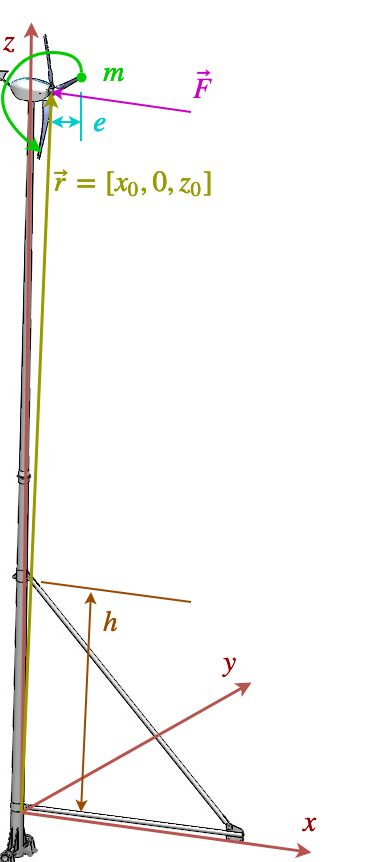
\includegraphics[scale=0.5]{annotated_tower}
	\decoRule
	\caption{The simplified wind turbine model showing the forces from an eccentric mass on the rotor.  This figure also shows the coordinate system that will be used for the tower analysis and is created using a Draw.io overlay on a SolidWorks model.}
	\label{fig:annotated_tower}
\end{figure}

%----------------------------------------------------------------------------------------
%	VARIABLE DEFINITIONS
%----------------------------------------------------------------------------------------

\section{Variable Definitions}

\begin{table}[] \label{t:variable_definitions}
\caption{Variable Definitions}
\vspace*{0.2in}
\begin{tabular}{|m{1in}|m{4in}|}
\hline
\rowcolor[HTML]{EFEFEF} 
\textbf{Variable} & \textbf{Description} \\ \hline
$\vec{F}_{original}$ & The original force applied to the end of the rotor due to an imbalance in the blades \\ \hline
$F_0$ & The magnitude of the force caused by the eccentric mass \\ \hline
$\omega$ & The rotational speed of the blades \\ \hline
$t$ & Time \\ \hline
$m$ & Eccentric mass \\ \hline
$e$ & Distance the eccentric mass is from the axis of rotation of the rotor \\ \hline
$\vec{M}$ & Moment that the eccentric force applies after the force is translated to the tower axis \\ \hline
$\vec{r}$ & The position vector for the top of the rotor with respect to the bottom of the turbine tower ($r=[x_0, 0, z_0]$) \\ \hline
$M_x$ & The moment function in the $x$-direction \\ \hline
$M_y$ & The moment function in the $y$-direction \\ \hline
$I_b$ & The area moment of inertia at the base of the tower \\ \hline
$I_t$ & The area moment of inertia at the top of the tower \\ \hline
$h$ & The distance from the base of the tower to the ginpole pin-joint on the tower \\ \hline
$E$ & Modulus of elasticity of the tower (steel) \\ \hline
$d_b$ & Diameter at the base of the tower \\ \hline
$d_t$ & Diameter at the top of the tower \\ \hline
\end{tabular}
\end{table}
\FloatBarrier



%----------------------------------------------------------------------------------------
%	CALCULATING TOWER VIBRATIONS
%----------------------------------------------------------------------------------------

\section{Calculating Tower Vibrations}

\subsection{Determining Effective Force}

An eccentric mass, $m$, on the rotor causes a force defined by the following equation:

\begin{equation} \label{eq:initial_force}
	\vec{F}(t) = 
		\begin{bmatrix}
			0 \\
			F_0\sin{(\omega t)} \\
			F_0\cos{(\omega t)}	
		\end{bmatrix}
\end{equation}

where

\begin{equation}
	F_0 = me\omega^2
\end{equation}

In order to treat the system as a cantilever beam, the force has to be acting in the center of the nacelle and on the same axis as the tower.  When the force vector (Equation \ref{eq:initial_force}) is translated to the axis of the tower, a moment needs to be introduced to account for the force vector translation:

\begin{equation} \label{eq:translated_moment}
	\vec{M} = \vec{r} \times \vec{F} = 
		\begin{bmatrix}
			- F_{0} z_{0} \sin{\left (\omega t \right )}\\
			- F_{0} x_{0} \cos{\left (\omega t \right )}\\
			F_{0} x_{0} \sin{\left (\omega t \right )}
		\end{bmatrix}
\end{equation}

The moment in (Equation \ref{eq:translated_moment}) creates an effective force at the top of the tower that needs to be added to the original force (Equation \ref{eq:initial_force}).  The moment about the $z$-axis is ignored because torsional effects on the tower are negligible when determining nacelle displacement.  This results in the following effective force on the top of the tower:

\begin{equation}\label{eq:effective_force}
	\vec{F}_{effective} = \vec{F}_{original} + \vec{F}_{moment}
\end{equation}
$$ 
	\vec{F}_{effective} = 
	\begin{bmatrix}0\\F_{0} \sin{\left (\omega t \right )}\\F_{0} \cos{\left (\omega t \right )}\end{bmatrix}
	+ \begin{bmatrix}- \frac{F_{0} x_{0}}{z_{0}} \cos{\left (\omega t \right )}\\ F_{0} \sin{\left (\omega t \right )}\\ 0\end{bmatrix}
$$

\begin{equation}
	\vec{F}_{effective} = 
		\left[\begin{matrix}- \frac{F_{0} x_{0}}{z_{0}} \cos{\left (\omega t \right )}\\2 F_{0} \sin{\left (\omega t \right )}\\F_{0} \cos{\left (\omega t \right )}\end{matrix}\right]
\end{equation}

%----------------------------------------------------------------------------------------
%	DETERMINING EFFECTIVE SPRING CONSTANT
%----------------------------------------------------------------------------------------
\subsection{Determining Effective Spring Constant}
The tower model has a different spring constant for the $x$ and $y$ directions.  In the $y$ direction, the ginpole has a negligible effect on the stiffness of the tower, so the tower acts as a tapered cantilever beam. 


%	Deriving the y-direction spring constant
%----------------------------------------------------------------------------------------
\subsubsection{Mathematical derivation of the $y$-direction spring constant, $K_y$}
Assuming the tower acts like a cantilever beam in this direction with a concentrated force at the end of the beam, the moment, $M_x(y)$ can be expressed as:

\begin{equation} \label{eq:moment}
	M_x(y) = F_{y}\,z-F_{y}\,z_{0}
\end{equation}

Because the beam is linearly tapered, the diameter, $d$, can be written as a function of tower height, $z_0$.

\begin{equation} \label{eq:diameter_eq}
	d(z) = d_{b}-\frac{z\,\left(d_{b}-d_{t}\right)}{z_{0}}
\end{equation}

$d_b$ is the diameter of the tower at the bottom, and $d_t$ is the diameter of the tower at the top.  The moment of inertia, assuming a hollow tube with thickness $t$, can be written as a function of $z$ using Equation \ref{eq:diameter_eq}.

\begin{align}
	I_y(z) &= \frac{\pi}{64}d^4 - \frac{\pi}{64}\left(d-2t \right)^4 \\
	I_y(z) &= \frac{\pi \,{\left(d_{b}-\frac{z\,\left(d_{b}-d_{t}\right)}{z_{0}}\right)}^4}{64}-\frac{\pi \,{\left(2\,t-d_{b}+\frac{z\,\left(d_{b}-d_{t}\right)}{z_{0}}\right)}^4}{64} \label{eq:y_moment_intertia}
\end{align}

The deflection of the beam can be calculated using the Euler–Bernoulli equation:

\begin{align}
	\frac{d^2 y_d}{dz^2} &= -\frac{M_x}{E\,I_y(z)} \\
	\frac{d^2 y_d}{dz^2} &= -\frac{F_{y}\,z-F_{y}\,z_{0}}{E\,\left(\frac{\pi \,{\left(d_{b}-\frac{z\,\left(d_{b}-d_{t}\right)}{z_{0}}\right)}^4}{64}-\frac{\pi \,{\left(2\,t-d_{b}+\frac{z\,\left(d_{b}-d_{t}\right)}{z_{0}}\right)}^4}{64}\right)}
 \label{eq:curvature_eq_y}
\end{align}

The slope of the beam, $\theta_y$, can be calculated by integrating Equation \ref{eq:curvature_eq_y}:

\begin{equation}
	\theta_y = \frac{dy_d}{dz} = \int{-\frac{F_{y}\,z-F_{y}\,z_{0}}{E\,\left(\frac{\pi \,{\left(d_{b}-\frac{z\,\left(d_{b}-d_{t}\right)}{z_{0}}\right)}^4}{64}-\frac{\pi \,{\left(2\,t-d_{b}+\frac{z\,\left(d_{b}-d_{t}\right)}{z_{0}}\right)}^4}{64}\right)}\,dz}
\end{equation}

Integrating the equation above results in the following equation for $\theta_y$:

\begin{align}
	\theta_y =\, &\frac{\ln\left(d_{b}\,z-d_{t}\,z-d_{b}\,z_{0}+t\,z_{0}\right)\,\left(8\,F_{y}\,d_{t}\,{z_{0}}^2-8\,F_{y}\,t\,{z_{0}}^2\right)}{E\,\pi \,{d_{b}}^2\,t^3-2\,E\,\pi \,d_{b}\,d_{t}\,t^3+E\,\pi \,{d_{t}}^2\,t^3} \nonumber \\
	&-\frac{4\,\ln\left(d_{b}\,z-d_{t}\,z-d_{b}\,z_{0}+t\,z_{0}\,\left(1-\mathrm{i}\right)\right)\,\left(F_{y}\,d_{t}\,{z_{0}}^2+F_{y}\,t\,{z_{0}}^2\,\left(-1+1{}\mathrm{i}\right)\right)}{E\,\pi \,{d_{b}}^2\,t^3-2\,E\,\pi \,d_{b}\,d_{t}\,t^3+E\,\pi \,{d_{t}}^2\,t^3} \nonumber \\
	&-\frac{4\,\ln\left(d_{b}\,z-d_{t}\,z-d_{b}\,z_{0}+t\,z_{0}\,\left(1+1{}\mathrm{i}\right)\right)\,\left(F_{y}\,d_{t}\,{z_{0}}^2+F_{y}\,t\,{z_{0}}^2\,\left(-1-\mathrm{i}\right)\right)}{E\,\pi \,{d_{b}}^2\,t^3-2\,E\,\pi \,d_{b}\,d_{t}\,t^3+E\,\pi \,{d_{t}}^2\,t^3} + C_{y1}
\end{align}


The tower is fixed at the base (no translation or rotation about the $x$-axis), so the slope at $z=0$ is $\theta=0$.  Using this boundary condition, $C_{y1}$ can be determined:
\begin{align}
	C_{y1} = -\frac{4\,F_{y}\,{z_{0}}^2\,Q_1(z)}{E\,t^3\,\pi \,{\left(d_{b}-d_{t}\right)}^2}
\end{align}

where, 
\begin{align*}
	Q_1(z) =\, &2\,d_{t}\,\ln\left(-z_{0}\,\left(d_{b}-t\right)\right)-d_{t}\,\ln\left(-z_{0}\,\left(d_{b}+t\,\left(-1-\mathrm{i}\right)\right)\right) \\
	&-d_{t}\,\ln\left(-z_{0}\,\left(d_{b}+t\,\left(-1+1{}\mathrm{i}\right)\right)\right)-2\,t\,\ln\left(-z_{0}\,\left(d_{b}-t\right)\right) \\
	&+t\,\ln\left(-z_{0}\,\left(d_{b}+t\,\left(-1-\mathrm{i}\right)\right)\right)\,\left(1+1{}\mathrm{i}\right) \\
	&+t\,\ln\left(-z_{0}\,\left(d_{b}+t\,\left(-1+1{}\mathrm{i}\right)\right)\right)\,\left(1-\mathrm{i}\right)
\end{align*}

This results in the following slope equation:

\begin{align} \label{eq:theta_analytic}
	\theta_y = \frac{4\,F_{y}\,{z_{0}}^2\,Q_2(z)}{E\,t^3\,\pi \,{\left(d_{b}-d_{t}\right)}^2} + C_{y1}
\end{align}

where,
\begin{align*}
	Q_2(z) =\, &2\,d_{t}\,\ln\left(d_{b}\,z-d_{t}\,z-d_{b}\,z_{0}+t\,z_{0}\right) \\
	&-d_{t}\,\ln\left(d_{b}\,z-d_{t}\,z-d_{b}\,z_{0}+t\,z_{0}\,\left(1-\mathrm{i}\right)\right) \\
	&-d_{t}\,\ln\left(d_{b}\,z-d_{t}\,z-d_{b}\,z_{0}+t\,z_{0}\,\left(1+1{}\mathrm{i}\right)\right) \\
	&-2\,d_{t}\,\ln\left(-z_{0}\,\left(d_{b}-t\right)\right)+d_{t}\,\ln\left(-z_{0}\,\left(d_{b}+t\,\left(-1-\mathrm{i}\right)\right)\right) \\
	&+d_{t}\,\ln\left(-z_{0}\,\left(d_{b}+t\,\left(-1+1{}\mathrm{i}\right)\right)\right) \\
	&-2\,t\,\ln\left(d_{b}\,z-d_{t}\,z-d_{b}\,z_{0}+t\,z_{0}\right) \\
	&+t\,\ln\left(d_{b}\,z-d_{t}\,z-d_{b}\,z_{0}+t\,z_{0}\,\left(1-\mathrm{i}\right)\right)\,\left(1-\mathrm{i}\right) \\
	&+t\,\ln\left(d_{b}\,z-d_{t}\,z-d_{b}\,z_{0}+t\,z_{0}\,\left(1+1{}\mathrm{i}\right)\right)\,\left(1+1{}\mathrm{i}\right) \\
	&+2\,t\,\ln\left(-z_{0}\,\left(d_{b}-t\right)\right)+t\,\ln\left(-z_{0}\,\left(d_{b}+t\,\left(-1-\mathrm{i}\right)\right)\right)\,\left(-1-\mathrm{i}\right) \\
	&+t\,\ln\left(-z_{0}\,\left(d_{b}+t\,\left(-1+1{}\mathrm{i}\right)\right)\right)\,\left(-1+1{}\mathrm{i}\right)
\end{align*}

At this point, it has become clear that an analytic solution for the spring constant is not practical.  Integrating the slope equation (Equation \ref{eq:theta_analytic}) would produce the deflection equation; however this integral become extremely complicated.  A cleaner option is to calculate the spring constants numerically.

\subsubsection{Numerical calculation of the $y$-direction spring constant, $K_y$}
To determine the spring constant numerically, a vector of $z$ values must be created to be used in the numerical integration. 

To calculate the slope of the tower, $\theta$, the curvature equation needs to be numerically integrated:

\begin{equation}
	\theta(z) = \int_0^{z_0}{\frac{-M(z)}{E\,I(z)}\,dz}
\end{equation}

The applied force, $F_y$, in the moment equation (Equation \ref{eq:moment}) can be factored out because it is not a function of $z$.  This results in the following equation for the slope:

\begin{equation} \label{eq:theta_integral_exact}
	\theta(z) = \frac{F_y}{E} \int_0^{z_0}{\frac{z_0-z}{I(z)}\,dz}
\end{equation}

The integral in Equation \ref{eq:theta_integral_exact} can be approximated by a sum of $n$ elements and calculated numerically.

\begin{equation} \label{eq:theta_integral_approx}
	\theta(z) = \frac{F_y}{E} \sum_{i=0}^{n}{\frac{z_0-z_i}{I(z_i)}\,\Delta z_i}
\end{equation}

Equation \ref{eq:theta_integral_approx} is a much simpler method for calculating the beam slope compared to the analytic solution shown in Equation \ref{eq:theta_analytic}.  The deflection of the tower, $y_d$, can be calculated by integrating the slope equation.

\begin{equation}
	y_d = \int_{0}^{z_0}{\theta(z)\,dz} = \int_{0}^{z_0}{\left(\frac{F_y}{E} \sum_{i=0}^{n}{\frac{z_0-z_i}{I(z_i)}\,\Delta z_i}\right)dz}
\end{equation}

The above equation can be numerically approximated with a summation of $m$ elements as follows:

\begin{align}
	y_d &= \sum_{j=0}^{m}{\left(\frac{F_y}{E} \sum_{i=0}^{n}{\frac{z_0-z_{ij}}{I(z_{ij})}\,\Delta z_i}\right) \Delta z_j} \\
	y_d &= \frac{F_y}{E}\sum_{j=0}^{m}{\sum_{i=0}^{n}{\frac{z_0-z_{ij}}{I(z_{ij})}\,\Delta z_i} \Delta z_j} \label{eq:deflection_equation_sum}
\end{align}

To determine the spring constant, the deflection equation should be rewritten in the form, $F=-kx$, which in this case is:
\begin{align}
	F_y &= -k_y \, y_d \\
	F_y &= \frac{E}{\sum_{j=0}^{m}{\sum_{i=0}^{n}{\frac{z_{ij}-z_0}{I(z_{ij})}\,\Delta z_i} \Delta z_j}} \, y_d \label{eq:Fy_numerical}
\end{align}

From Equation \ref{eq:Fy_numerical}, is can be seen that the spring constant is:
\begin{equation} \label{eq:ky}
	k_y = \frac{E}{\sum_{j=0}^{m}{\sum_{i=0}^{n}{\frac{z_{ij}-z_0}{I(z_{ij})}\,\Delta z_i} \Delta z_j}}
\end{equation}


\begin{table}[]
\caption{Calculated spring constant and natural frequency for the $y$-direction vibration.} \label{t:ky_values}
\begin{center}
\begin{tabular}{|m{1in}|m{1in}|m{1in}|m{1in}|m{1in}|}
\rowcolor[HTML]{EFEFEF} 
\hline
\textbf{Parameter} & \textbf{Constant Top Area} & \textbf{Tapered Beam} & \textbf{Constant Bottom Area} & \textbf{FEA value} \\ \hline
$k_y$ & 1283 N/m & 8966 N/m & 16213 N/m & 8159 N/m \\  \hline
$f_y$ & 0.34 Hz & 0.61 Hz & 1.1 Hz & 0.58 Hz\\ \hline
\end{tabular}
\end{center}
\end{table}

Table \ref{t:ky_values} shows the calculated spring constant values and natural frequencies in the $y$-direction for the turbine parameters.  The constant top area value is the spring constant calculated assuming a uniform circular cross-section beam with a profile equal to the top of the tower.  The constant bottom area value is the spring constant calculated assuming a uniform circular cross-section beam with a profile equal to the bottom of the tower.  The FEA values are derived in Tom Gwon's analysis \cite{Gwon_paper}, although it is unclear whether these values apply for the $y$ or $x$ direction.  The tapered beam calculation is performed in MATLAB using the following code (with turbine parameters listed in Table \ref{t:MATLAB_ky_variables}):

\begin{lstlisting}
z = linspace(0, z_0, 1000); % [m] Create the vector of z values
M_F = (z - z_0); % [m] The moment equation with respect to the applied force (M/F)
d_F = d_b - z*(d_b-d_t)/z_0; % [m] The diameter as a function of height
I = pi/64*d.^4 - (pi/64)*(d-2*t).^4; % [m^4] The moment of inertia
v_F = -M_F ./ (E*I); % [s^2/m^2/kg] The curvature equation
theta_F = cumtrapz(z, v_F); % [s^2/m/kg] The slope equation
y_F = cumtrapz(z, theta_F); % [m/N] The displacement with respect to force
ky = 1 ./ y_F(end); % [N/m] Spring constant
\end{lstlisting}
\FloatBarrier


\begin{table}[]
\caption{Turbine parameters used in the MATLAB analysis for calculating $k_y$}
\label{t:MATLAB_ky_variables}
\vspace*{0.2in}
\begin{tabular}{|m{1in}|m{1in}|m{4in}|}
\hline
\rowcolor[HTML]{EFEFEF} 
\textbf{Variable} & \textbf{Value} & \textbf{Description} \\ \hline
$z_0$ & 70 ft & The total height of the tower \\ \hline
$d_b$ & 20 in & The diameter of the bottom of the tower \\ \hline
$d_t$ & 8.7 in & The diameter of the top of the tower \\ \hline
$E$ & 30 Mpsi & The modulus of elasticity for ASTM A572 Grade-50 Steel \\ \hline
$t$ & 0.2 in & The thickness of the turbine tower tube \\ \hline
\end{tabular}
\end{table}

The intermediate variables from the MATLAB calculation are shown in Figure  \ref{fig:ky_MATLAB_plot}.  The curvature, slope, and displacement are all with respect to force, since it cancels out of the equation and is not used.  The spring constant is calculated by taking the inverse of the displacement/force curve at the largest $z$ value.  These plots were created using a $z$-vector of 1000 elements.

\begin{figure}
	\centering
	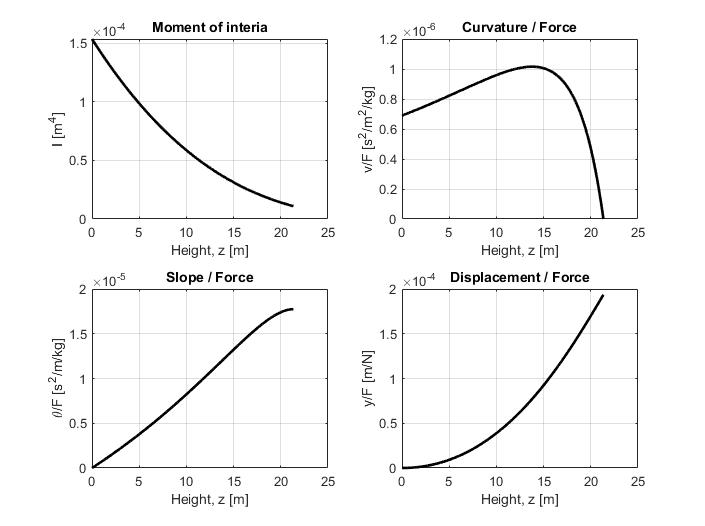
\includegraphics[scale=0.7]{ky_MATLAB_plot}
	\decoRule
	\caption{The intermediate variables from the numerical spring constant calculation in MATLAB.}
	\label{fig:ky_MATLAB_plot}
\end{figure}
\FloatBarrier


%----------------------------------------------------------------------------------------
%	DETERMINING EFFECTIVE MASS
%----------------------------------------------------------------------------------------

\subsection{Determining Effective Mass}
The cantilever beam (Figure \ref{fig:cantilever_beam}) can be simplified to a massless beam with all of the mass concentrated at the end of the beam.

% Figure for the cantilever beam
\begin{figure}
	\centering
	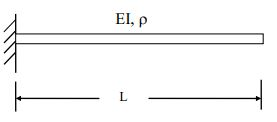
\includegraphics[scale=1]{cantilever_beam}
	\decoRule
	\caption{A cantilever beam model \cite{cantilever_beam_ref}}
	\label{fig:cantilever_beam}
\end{figure}

As shown in Figure \ref{fig:ky_MATLAB_plot}, the deflection at any point on the beam, $y(z)$ can be calculated numerically.  The normalized deflection, $y_n(z)$ can be calculated by dividing this equation by the maximum deflection at the free end, $z_0$ (Equation \ref{eq:normalized_deflection}).  This allows the deflection equation to be rewritten in terms of the normalized deflection (Equation \ref{eq:deflection_w_normalization}).
\begin{align}
	y_n(z) &= \frac{y(z)}{y(z_0)} \label{eq:normalized_deflection} \\
	y(z) &= y_n(z) \cdot y(z_0) = y_n(z) \cdot y_{max} \label{eq:deflection_w_normalization} \\
\end{align}

The velocity of the beam at point $z$ can be calculated by taking the derivative of the deflection equation (Equation \ref{eq:deflection_w_normalization}).  The velocity of the beam is shown in Equation \ref{eq:beam_velocity}.
\begin{equation} \label{eq:beam_velocity}
	v(z) = y_n(z) \cdot v_{max}
\end{equation}

The kinetic energy, $dE_k$, of the beam at a single point, $x$, can be calculated as shown in Equation \ref{eq:beam_ke}.
\begin{align}
	dE_k &= \frac{1}{2} m v^2 \nonumber \\
	dE_k &= \frac{1}{2} \left(\rho A(z) dz\right) \left(y_n(z) v_{max}\right)^2  \label{eq:beam_ke}
\end{align}

Using Equation \ref{eq:beam_ke}, the total kinetic energy of the beam can be found by integrating $dE_k$, as shown in Equation \ref{eq:beam_ke_total}.
\begin{align}
	E_k &= \int_{0}^{z_0}{dE_k} \\
	E_k &= \int_{0}^{z_0}{\left(\frac{1}{2} \rho A(z) \left(y_n(z) v_{max}\right)^2 dz \right)} \\
	E_k &= \frac{1}{2} \rho v_{max}^2 \int_{0}^{z_0}{\left(A(z) y_n^2(z) dz \right)} \label{eq:beam_ke_total}
\end{align}

The effective mass of the beam can be calculated by examining Equation \ref{eq:beam_ke_total} and comparing to the standard format, $E=\frac{1}{2}mv^2$.  Equation \ref{eq:effective_mass_integral} shows the resulting effective mass.
\begin{equation} \label{eq:effective_mass_integral}
	m_{eff} = \rho \int_{0}^{z_0}{\left(A(z) y_n^2(z) dz \right)}
\end{equation}

The deflection from Equation \ref{eq:deflection_equation_sum} can be substituted into Equation \ref{eq:effective_mass_integral}.  Additionally, the integral can be converted to a numerical sum as shown in Equation \ref{eq:m_eff_sum}.
\begin{equation} \label{eq:m_eff_sum}
	m_{eff} = \rho \sum_{k=0}^{p}{\left(A(z_p) y_n^2(z_p) \Delta z \right)}
\end{equation}

Numerically calculating $m_{eff}$ using MATLAB, results in a value of $m_{eff}=140 \units{kg}$.

The total effective mass at the top of the tower, $m_{eff,total}$ is as follows:
\begin{align}
	m_{eff,total} &= m_{nacelle} + m_{eff} \\
	m_{eff,total} &= 474 \units{kg} + 140 \units{kg} = 614 \units{kg} \label{eq:total_effective_mass}
\end{align}

The mass in Equation \ref{eq:total_effective_mass} is the lumped sum used to calculate the  parameters in Table \ref{t:ky_values} and create the turbine tower model.

\subsection{Developing State Space Equations}
Vibrations in the $x$ and $y$ directions can be split up into 2 independent 2nd order differential equations:
\begin{align}
	\ddot{x} + \frac{C_x}{m} \dot{x} + \frac{k_x}{m} x = \frac{1}{m} F_x(t) \\
	\ddot{y} + \frac{C_y}{m} \dot{y} + \frac{k_y}{m} x = \frac{1}{m} F_y(t)
\end{align}

These equations can be converted to state space form:
\begin{align}
	&\bm{\dot{x}} = \bm{A_x} \bm{x} + \bm{B_x} F_x(t) \\
	&x = \bm{C_x} \bm{x} + \bm{D_x} F_x(t) \\
	&\bm{\dot{y}} = \bm{A_y} \bm{y} + \bm{B_y} F_y(t) \\
	&y = \bm{C_y} \bm{y} + \bm{D_y} F_y(t)
\end{align}

Where the full equations are written out as follows:
\begin{align}
	\begin{bmatrix}
		\dot{x}_1 \\
		\dot{x}_2
	\end{bmatrix} = 		
	\left[\begin{matrix}0 & 1\\- \frac{k_{x}}{m} & - \frac{C_{x}}{m}\end{matrix}\right]
	\left[\begin{matrix}x_{1} \\ x_{2}\end{matrix}\right] +
	\left[\begin{matrix}0 \\ \frac{1}{m}\end{matrix}\right] \cdot F_x(t)\\
	x=
	\begin{bmatrix}
		1 & 0
	\end{bmatrix}
	\begin{bmatrix}
		x_1 \\ x_2		
	\end{bmatrix} + 0 \cdot F_x(t)
\end{align}

\begin{align}
	\begin{bmatrix}
		\dot{y}_1 \\
		\dot{y}_2
	\end{bmatrix} = 		
	\left[\begin{matrix}0 & 1\\- \frac{k_{y}}{m} & - \frac{C_{y}}{m}\end{matrix}\right]
	\left[\begin{matrix}y_{1} \\ y_{2}\end{matrix}\right] +
	\left[\begin{matrix}0 \\ \frac{1}{m}\end{matrix}\right] \cdot F_y(t)\\	
	y=
	\begin{bmatrix}
		1 & 0
	\end{bmatrix}
	\begin{bmatrix}
		y_1 \\ y_2		
	\end{bmatrix} + 0 \cdot F_y(t)	
\end{align}

These equations are for a simple cantilever model with a lumped mass at the end of the beam (lumped mass accounts for nacelle and tower mass).  The resulting natural frequency from this model matches the ABAQUS FEA results from Gwon's paper \cite{Gwon_paper}.  A comparison between the resulting natural frequency from this model and the ABAQUS FEA results in Gwon's analysis \cite{Gwon_paper} can be seen in Table \ref{t:ky_values}.